\section{Проектирование модификаций программного средства} % (fold)
\label{sec:development}

Как уже было отмечено, данная работа представляет собой модификацию существующего программного средства, разработанного в рамках дипломного проекта.

В разделе ~\ref{sec:development:common} будет представлен общий список модификаций, выполненных в рамках работы,
и причины по которым данные модификации были необходимы.

Напомним, что программное средство состоит из трех независимых модулей:

\begin{itemize}
  \item модуль чтения и разбора схемы сооружения и сценария симуляции;
  \item модуль выполнения симуляции;
  \item модуль отображения результатов симуляции.
\end{itemize}

Модули обмениваются данными в определенном бинарном формате.

Первый модуль отвечает за разбор всей конфигурации симуляции и формирование бинарного сообщения о конфигурации второму модулю.
Данный модуль написан на языке программирования Ruby~\cite{ruby_doc}, и представляет собой имплементацию предметно"=ориентированного языка описания сценария симуляции.
Модуль не претерпевал значительных изменений в рамках разработки модификации по учету сценария массовой паники,
однако немногие изменения будут описаны в разделе~\ref{sec:development:preprocessor}.

Второй модуль является ядром программного средства, и большинство модификаций требовали изменений в этом модуле.
Написан он на языке программирования Rust~\cite{rust_doc}, и представляет собой реализацию теоретической модели пешеходных потоков.
В рамках данной работы в этот модуль была добавлена теоретическая модель поведения пешеходов в сценарии массовой паники.
Конкретные изменения будут описаны в разделе~\ref{sec:development:core}.

Последний модуль используется для отображения результатов симуляции на экране,
и написан на языке программирования C с использованием библиотеки SDL~\cite{libsdl_home}.
Список изменений, внесенных в данный модуль, можно найти в разделе~\ref{sec:development:animator}.

\subsection{Модификации программного средства}
\label{sec:development:common}

В первую очередь разрабатываемое программное средство должно реализовывать описанную в разделе~\ref{sec:model} модель паники.
Для этого необходимо внести изменения в вычисление различных социальных сил, ввести новые социальные силы,
а также добавить имплементацию модели распространения паники.
Все эти модификации касаются модуля выполнения симуляции, и будут подробно обсуждены в разделе~\ref{sec:development:core}.

Однако можно заметить, что режим работы существующего программного средства не совсем подходит для демонстрации эффектов паники.

Существующее программное средство работает в режиме <<потока>>.
На схеме сооружения существуют области появления людей (обычно располагаются на границах схемы),
генерирующие с определенной частотой новых пешеходов.
Каждый пешеход имеет набор промежуточных целей и одну конечную цель, по достижении которой он исчезает.
Таким образом генерируются непрекращающиеся <<потоки>> пешеходов от области появления до конечных целей.

И хотя данный режим позволяет оценить эффекты паники на поток пешеходов, намного более интересным является сценарий эвакуации.
В сценарии эвакуации существует определенное заранее заданное количество людей внутри сооружения.
В начале симуляции каждый пешеход находится в определенном месте, и с началом симуляции пытается добраться до выхода из здания.
Симуляция завершается, когда последний пешеход достигает своей цели.
В данном сценарии эффекты паники будут проявляться намного более наглядно, что позволит лучше их продемонстрировать.

По описанным выше причинам было решено внести в программное средство модификации,
которые позволяли бы проводить симуляцию по сценарию эвакуации
(в дальнейшем данный режим работы будем называть режимом эвакуации).
При этом важными параметрами в данном режиме являются статистические характеристики
итогового времени эвакуации для набора пешеходов, такие как минимальное и максимальное время эвакуации,
среднее время эвакуации, дисперсия времени эвакуации "---
разрабатываемое программное средство должно вычислять данные характеристики и представлять их пользователю.
Изменения, требуемые для реализации описанного режима эвакуации, были внесены во все три модуля программного средства,
и будут описаны в разделах~\ref{sec:development:preprocessor:escape}, \ref{sec:development:core:escape} и \ref{sec:development:animator:escape}.


\subsection{Модификации модуля чтения и разбора схемы сооружения и сценария симуляции}
\label{sec:development:preprocessor}

Как уже было отмечено, модуль чтения и разбора схемы сооружения и сценария симуляции не требовал значительных модификаций.

Напомним, что сценарий симуляции имеет вид, представленный на рисунке рисунке~\ref{sec:development:preprocessor:scenario_dsl_listing}.

\begin{figure}[ht!]
  \centering
  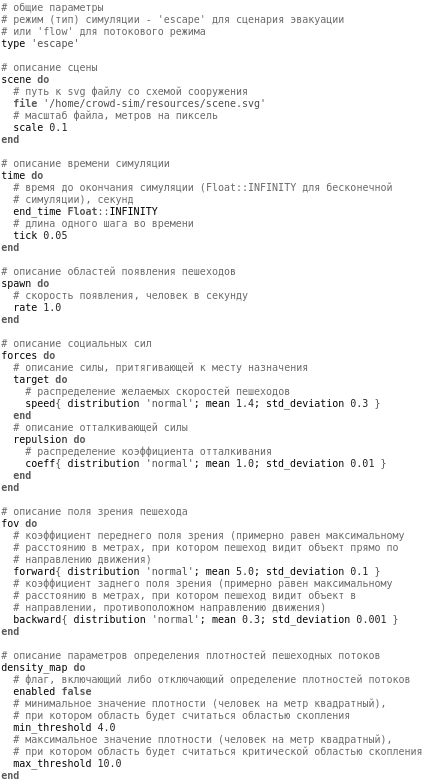
\includegraphics[width=\dimexpr\linewidth-4.5em\relax]{masters_sim_params_example}
  \caption{Пример сценария симуляции}
  \label{sec:development:preprocessor:scenario_dsl_listing}
\end{figure}

В модуль были внесены всего две модификации: поддержка различных режимов симуляции (задаются в сценарии симуляции) и поддержка источников паники (задаются в схеме сооружения).
Первая модификация описана в разделе~\ref{sec:development:preprocessor:escape}, а вторая "--- в разделе~\ref{sec:development:preprocessor:panic_source}.

\subsubsection{Режимы симуляции в сценарии симуляции}
\label{sec:development:preprocessor:escape}

В конфигурации сценария симуляции каждый параметр принадлежит определенной секции и имеет определенный номер.
Соответственно, изменение сводилось к добавлению нового параметра в секцию и присвоение ему номера.
Так как данный параметр (<<режим симуляции>>) не подходил по смыслу ни в одну существующую секцию,
для него была создана новая секция под названием <<Общие параметры>>.

Также для данного поля был введен новый тип "--- перечисление.
Данный тип позволяет указывать в сценарии симуляции строку, соответствующую набору заранее определенных строк.
При этом если строка не была найдена в заранее определенном наборе, сценарий симуляции считается неверным и выдается ошибка.
При генерировании сообщения о конфигурации элементы полей данного типа преобразуют строку в целую константу, что упрощает чтение и разбор на стороне модуля выполнения симуляции.

Таким образом, новое поле принадлежит секции <<Общие параметры>>,
и имеет тип перечисление с возможными значениями "flow" (потоковая симуляция) и
"escape" (симуляция в режиме эвакуации).

Напомним, что бинарный формат описания конфигурации (результат работы модуля, передающийся модулю выполнения симуляции)
состоит из отдельных независимых друг от друга элементов.
Каждый элемент имеет следующую структуру:
\begin{itemize}
  \item идентификатор секции, к которой принадлежит данный элемент (1 байт);
  \item идентификатор элемента внутри данной секции (2 байта);
  \item данные элемента, закодированные в бинарном формате (переменное количество байт).
\end{itemize}

Таким образом, подробно новый элемент конфигурации можно представить в виде таблицы~\ref{sec:development:preprocessor:format_table_escape}.

\begin{longtable}[ht]{| >{\centering}m{0.25\textwidth}
                      | >{\centering}m{0.25\textwidth}
                      | >{\centering\arraybackslash}m{0.40\textwidth}|}
\caption{Формат сообщения о конфигурации "--- режим симуляции} \label{sec:development:preprocessor:format_table_escape}\tabularnewline

\hline Секция & Элемент & Данные элемента \tabularnewline
\endfirsthead
\captionsetup{labelformat=stbtablecont,justification=raggedright}
\caption[]{}\tabularnewline
\hline 1 & 2 & 3 \tabularnewline
\endhead
  \hline Общие параметры "--- 0x00 & Режим симуляции "--- 0x0001 & \specialcell{тип (целое, 1 байт)\\
                                                                                0x01 "--- потоковая симуляция\\
                                                                                0x02 "--- симуляция сценария\\
                                                                                эвакуации}\tabularnewline
  \hline
\end{longtable}


\subsubsection{Источники паники в схеме сооружения}
\label{sec:development:preprocessor:panic_source}

В качестве схемы сооружения выступает особым образом модифицированный SVG~\cite{svg_home} файл.
SVG "--- распространенный формат векторной графики на основе XML.

Пример схемы сооружения представлен на рисунке~\ref{sec:development:preprocessor:svg_scheme_listing}.
Как видно из примера, все дополнительные параметры объектов добавлены в атрибуты с префиксом x-csim.

Для отображения источников паники была добавлена поддержка нового элемента SVG "--- circle,
атрибут x-csim-class у которого установлен в panic-source. Также у этого элемента есть дополнительный атрибут "--- x-csim-power,
задающий силу данного источника.

\begin{figure}[!htb]
  \centering
  \begin{subfigure}[!htb]{0.45\textwidth}
    \centering
    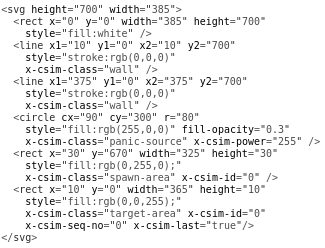
\includegraphics[scale=1.0]{masters_scene_example_text}
    \caption{}
  \end{subfigure}
  \begin{subfigure}[!htb]{0.45\textwidth}
    \centering
    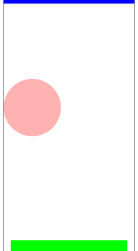
\includegraphics[scale=2.0]{masters_scene_example_pic}
    \caption{}
  \end{subfigure}
  \caption{Пример простой схемы сооружения: а "--- текстовый листинг схемы;
           б "--- схема в виде картинки}
  \label{sec:development:preprocessor:svg_scheme_listing}
\end{figure}

Описание нового элемента конфигурации, соответствующего источнику паники, можно найти в таблицe~\ref{sec:development:preprocessor:format_table_panic_source}.

\begin{longtable}[ht]{| >{\centering}m{0.25\textwidth}
                      | >{\centering}m{0.25\textwidth}
                      | >{\centering\arraybackslash}m{0.40\textwidth}|}
\caption{Формат сообщения о конфигурации "--- источник паники} \label{sec:development:preprocessor:format_table_panic_source}\tabularnewline

\hline Секция & Элемент & Данные элемента \tabularnewline
\endfirsthead
\captionsetup{labelformat=stbtablecont,justification=raggedright}
\caption[]{}\tabularnewline
\hline 1 & 2 & 3 \tabularnewline
\endhead
  \hline Сцена "--- 0x01 & Источник паники "--- 0x0004 & \specialcell{координаты центра\\
                                                                      (x, y)\\
                                                                      радиус (целое, 2 байта)\\
                                                                      сила (целое, 1 байт)}\tabularnewline
  \hline
\end{longtable}

\FloatBarrier

\subsection{Модификации модуля выполнения симуляции}
\label{sec:development:core}

Изменения, внесенные в модуль выполнения симуляции, можно разбить на несколько групп:

\begin{itemize}
  \item разбор новых параметров конфигурации;
  \item имплементация нового режима работы "--- режима эвакуации;
  \item внесение изменений в социальные силы в соответствии с моделью;
  \item добавление модели распространения паники;
  \item предоставление дополнительной информации модулю отображения результатов;
\end{itemize}

Каждая из этих групп будет описана в разделе \ref{sec:development:core:configuration},
\ref{sec:development:core:escape}, \ref{sec:development:core:forces},
\ref{sec:development:core:panic_spread}, \ref{sec:development:core:output} соответственно.


\subsubsection{Разбор новых параметров конфигурации}
\label{sec:development:core:configuration}

Разбор и сохранение конфигурации осуществляется подмодулем con\-fi\-gu\-ra\-ti\-on.
В соответствии с разделом~\ref{sec:development:preprocessor}
и таблицами~\ref{sec:development:preprocessor:format_table_escape} и~\ref{sec:development:preprocessor:format_table_panic_source},
в данном подмодуле была реализована поддержка новых параметров конфигурации.

Были добавлены функция par\-se\_ge\-ne\-ral\_item для чтения параметров из секции общих параметров,
описания необходимых структур данных для хранения новых параметров (перечисление Sim\-Ty\-pe, структура Sce\-ne\-Pa\-nicSo\-urce)
и организовано чтение новых элементов в соответствии с их идентификаторами.

\subsubsection{Режим эвакуации}
\label{sec:development:core:escape}

Как уже было описано в разделе~\ref{sec:development:common}, режим эвакуации отличается от потокового режима следующими особенностями:

\begin{itemize}
  \item создание новых пешеходов происходит один раз в начале симуляции;
  \item условием завершения симуляции является отсутствие пешеходов;
  \item необходимо выполнить подсчет статистических характеристик времени достижения цели пешеходами;
  \item данные характеристики должны быть переданы в модуль отображения результатов.
\end{itemize}

Перенос создания новых пешеходов на другой этап симуляции и замена условия завершения симуляции
тривиальны и не требуют обсуждения.

Важной задачей был подсчет статистических характеристик времени достижения цели пешеходами.
Для получения полного набора характеристик требовалось сохранить время достижения цели каждого пешехода в отдельности,
а затем проанализировать весь массив накопленных данных.

Хотя данный подход успешно работает при небольших массивах данных, в работе было принято решение использовать другой, инкрементальный подход.
Причиной принятия данного решения можно назвать устоявшуюся практику разработки программных систем, которая не поощряет
неконтролируемое разрастание операционных данных (а следовательно, и увеличение объема занимаемой оперативной памяти).
Также данное решение позволит в будущем проводить анализ больших массивов данных
(например анализ времени достижения цели в потоковой симуляции, длящейся значительный период времени).

Перейдем к описанию инкрементального подхода при расчете статистических данных.
Суть данного подхода в том, что вместо сохранения всех значений случайной величины сохраняются только ее аггрегационные параметры.
По завершению эксперимента некоторые характеристики случайной величины могут быть получены из сохраненных параметров.
Самым простым примером данного подхода является получение среднего значения путем инкрементального накопления суммы и количества элементов.

В работе также используется еще один подобный расчет для дисперсии, использующий известную формулу:

\begin{equation}
  \label{sec:development:core:escape:d_fm}
  D(X) = M(X^2) - M(X)^2
\end{equation}
\begin{explanation}
где & $ M(X) $ & математическое ожидание (среднее значение) случайной величины Х. \\
\end{explanation}

Таким образом, накапливая не только сумму значений случайно величины, но и сумму квадратов, в дальнейшем можно получить дисперсию случайно величины.

Для реализации описанного подхода был создан подмодуль sta\-ti\-stics, хранящий в себе состояние множества случайных величин.
При достижении пешеходом своей цели, подмодулю sta\-ti\-stics передается сообщение о времени достижения цели пешеходом.
В ответ на это подмодуль обновляет состояние случайной величины <<время достижения цели>>.
В состоянии сохраняются такие параметры, как минимальное и максимальное значение, сумма значений, сумма квадратов значений и количество значений.
Соответственно, по достижению конца симуляции модуль может выдать такие характеристики случайной величины, как
минимальное и максимальное значение, количество значений, среднее значение, дисперсия (и стандартное отклонение) значений.

Для передачи указанных характеристик модулю отображения результатов пришлось значительно переделать протокол взаимодействия данных двух модулей.
Подробнее об этой проблеме и путях ее решения будет рассказано в разделе~\ref{sec:development:core:output}.

\subsubsection{Изменения в социальных силах}
\label{sec:development:core:forces}

Модификации требовали две используемых социальных силы "--- сила отталкивания Re\-pul\-si\-on\-For\-ce и
сила флуктуаций Fluc\-tu\-a\-ti\-on\-For\-ce.

Изменения в силе отталкивания сводились к замене формул, используемых при расчете данной силы,
и добавлению двух новых <<отталкивающих>> сил физического контакта.

Изменения же в силе флуктуаций были более сложными в реализации.
Требовалось создать флуктуации, сохраняющиеся во времени "--- следовательно, требовалось где-то хранить такие флуктуации.
Логичнее всего казалось сохранять эти флуктуации в объекте пешехода.

Однако возникла проблема с используемой моделью заимствования языка программирования Rust.
Заимствования (получение ссылки) на объект в данном языке программирования бывают двух типов "---
с правом на модификацию и без права на модификацию.

Объекты социальных сил получали ссылки на все используемые объекты (объект пешехода и объект сцены)
без права на модификацию. Для того, чтобы изменить данный тип ссылок на ссылки с правом на модификацию,
требовались значительные изменения по всему проекту.

Чтобы избежать значительных изменений, было принято решение сохранять данные о текущих флуктуациях в самой силе флуктуации.
Для этого каждому пешеходу был назначен уникальный идентификатор, а в структуре силы флуктуации был создан ассоциативный
массив от уникального идентификатора пешехода к объекту флуктуации.
При возникновении флуктуации она сохранялась в данный ассоциативный массив и продолжала действовать до тех пор, пока ее
время действия не истекало и она не удалялась из ассоциативного массива.

Остальные изменения в силе флуктуаций также сводились к замене формул и логики расчета.

Стоит отметить, что хотя сохранение набора флуктуаций в объекте силы флуктуации сначала кажется не совсем хорошим решением
по сравнению с сохранением флуктуаций в объекте пешехода, на самом деле данное решение лучше, так как уменьшает связность
между подмодулями (правда, за счет незначительного снижения производительности "--- требуется дополнительное время на поиск
флуктуации в ассоциативном массиве по идентификатору пешехода).

Также требовалось добавить новую социальную силу <<стадного поведения>> "--- Her\-ding\-For\-ce.
Благодаря наличию аналога интерфейса в используемом языке программирования Rust, добавление новых сил в программное средство
сводится к добавлению одного модуля и регистрации его в модуле сил. Также следует отметить, что в соответствии с замечанием в
разделе~\ref{sub:model:herding} в качестве текущего вектора скорости движения берется вектор скорости движения на предыдущем
шаге.

\subsubsection{Модель распространения паники}
\label{sec:development:core:panic_spread}

Реализация модели распространения паники также было достаточно серьезным изменением.

Как уже было описано выше, потребовалось модифицировать протокол конфигурации и модуль разбора элементов конфигурации для
получения списка источников паники на схеме сооружения.
В дальнейшем данный список хранится в объекте Sce\-ne в отдельном поле для доступа и расчета параметров пешеходов.

В соответствии с моделью, в объект пешехода было добавлено поле уровня паники, имеющее тип вещественного числа от нуля до единицы.
В метод, осуществляющий обновление состояния всей модели, была добавлена логика по пересчету уровня паники для каждого пешехода
в зависимости от наличия в области видимости источника паники, от среднего значения уровня паники ближайших пешеходов и от предыдущего уровня паники.

Как и в случае с силой <<стадного поведения>>, данное моделью определение рекурсивно,
и на каждом шаге берутся значения уровня паники на предыдущем шаге.

Также для наглядной демонстрации распространения уровня паники информация о текущем уровне паники передается модулю отображения результатов.

\subsubsection{Изменения в формате протокола общения с модулем отображения результатов}
\label{sec:development:core:output}

Как было отмечено в разделе~\ref{sec:development:core:escape}, необходимо было передать модулю отображения результатов
статистические характеристики времени достижения цели пешеходов.

Проблема была в том, что главный цикл модуля отображения результатов не был рассчитан на получение различных типов сообщений.
Таким образом, модуль отображения результатов всегда ожидал сообщения одного и того же формата
(включающего в себя текущее время симуляции, положения всех пешеходов и, при наличии, параметры областей скопления).

Для решения данной проблемы были введены типы сообщений "--- каждое сообщение теперь начиналось с его типа.
Трем компонентам предыдущего формата были выделены три идентификатора типа:
0x00 для текущего времени симуляции, 0x01 для параметров всех пешеходов (положение, направление, и др.) и 0x02 для областей скоплений.
Также был добавлен четвертый тип, 0x03, для передачи статистических характеристик.

Соответствующие изменения были внесены в подмодуль out\-put "--- перед каждым сообщением посылался его тип,
и в конце симуляции посылалось одно сообщение с типом 0x03 и набором статистических характеристик.

Также изменения коснулись сообщения о параметрах всех пешеходов "--- для более наглядного отображения распространения паники,
для каждого пешехода теперь дополнительно передается его уровень паники.

\subsection{Модификации модуля отображения результатов симуляции}
\label{sec:development:animator}

Как было отмечено в предыдущем разделе, главный цикл модуля отображения результатов симуляции подвергся изменениям.
Вместо чтения целиком нового состояния симуляции, главный цикл пытается прочитать одно сообщение за раз.

В случае, если модуль получает сообщение с типом <<статистические характеристики времени достижения цели>>, симуляция считается завершенной.
После данного события модуль переходит в новый цикл, в котором генерирует текстовое представление статистических характеристик,
выводит данное текстовое представление на экран и ожидает событие ввода для завершения работы.

Текстовое сообщение генерируется с помощью библиотеки SDL\_ttf~\cite{libsdl_ttf_home}, и имеет формат
"Simulation done!\\nTravel time statistics: min=\%.2f, max=\%.2f, count=\%d, avg=\%.2f, variance=\%.2f, std\_deviation=\%.2f\\nPress spacebar to exit",
где вместо шаблонов \%.2f и \%d подставляются реальные значения характеристик времени достижения цели.
Затем данное сообщение преобразуется в текстуру и выводится поверх экрана симуляции.  После нажатия на пробел модуль завершает работу.

Пример текстового сообщения о статистических характеристиках времени достижения цели представлен на рисунке~\ref{sec:development:animator:statistics_example}.

\begin{figure}[!ht]
  \centering
  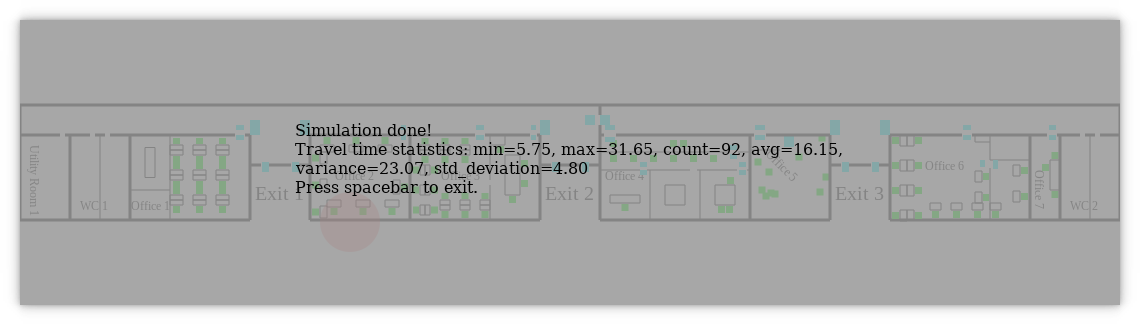
\includegraphics[width=\linewidth]{statistics_example}
  \caption{Пример отображения текстового сообщения со статистикой}
  \label{sec:development:animator:statistics_example}
\end{figure}

\begin{figure}[!ht]
  \centering
  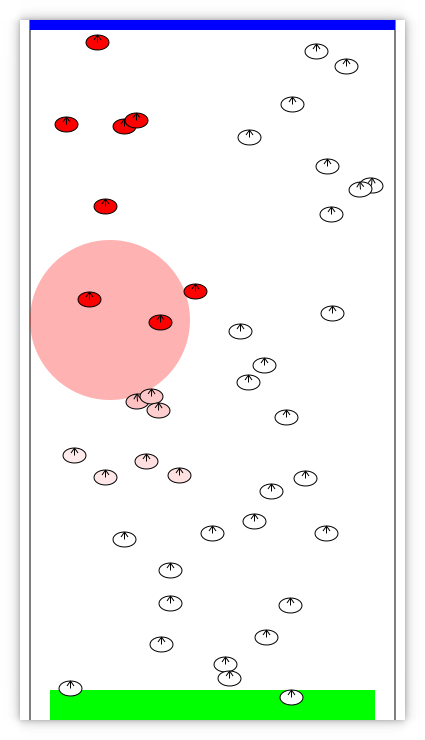
\includegraphics[scale=0.5]{panic_example}
  \caption{Пример отображения уровня паники пешеходов}
  \label{sec:development:animator:panic_example}
\end{figure}

Также модуль отображения результатов симуляции теперь отображает информацию об уровне паники каждого пешехода.
Чем выше уровень паники у конкретного пешехода, тем более его цвет смещается к красному.
Пример отображения пешеходов с высоким уровнем паники представлен на рисунке~\ref{sec:development:animator:panic_example}.


